\section{Mapas de Disparidade}
\label{sec:mapas_disparidade}

Os mapas de disparidade se tornaram uma ferramenta bastante utilizada para a
percepção tridimensional. Para robôs móveis autônomos os mapas de disparidade
são muito úteis, principalmente na detecção e desvio de obstáculos. O veículo
pode extrair uma informação de profundidade que servirá como parâmetro para a
navegação, por exemplo, uma região frontal de maior profundidade pode
representar um caminho sem obstáculos, livre de objetos e elementos localizados
em frente a câmera. Atualmente, a implementação direta em hardware dos
algoritmos de cálculo do mapa de disparidade a partir de um par de imagens
(câmera estéreo) permite a aplicação em tempo real e de forma embarcada
(\fig{fig:stoc_on_chip}) \cite{Khaleghi2008}.

A ideia fundamental do mapa de disparidade é fornecer uma informação de
profundidade relativa, mapeada diretamente na imagem bidimensional a partir do
valor do pixel. Usualmente são utilizadas imagens em tons de cinza (8
\textit{bits}), fornecendo então até 255 níveis de profundidade. Na
\fig{fig:tsukuba}, o mapa de disparidade está representando os obstáculos mais
próximos por tons mais claros e os obstáculos mais distantes por tons mais
escuros. Desta forma, os pixeis da imagem passam a representar no lugar da
informação de cor ou luminosidade uma informação de profundidade sobre os
elementos da cena. Os dispositivos sensores que fornecem uma imagem colorida
juntamente com o mapa de disparidade têm sido denominados de dispositivos RGB-D
(Imagem RGB + \textit{Depth}/mapa de disparidade). O sensor Kinect da
Microsoft\foot{Microsoft Kinect - http://www.xbox.com/en-us/kinect} fornece
imagens RGB-D com uma precisão de 2047 níveis de profundidade. Uma avaliação da
qualidade do mapa de disparidade produzido pelo Kinect \cite{Khoshelham2012}
mostrou que a relação entre o nível de profundidade e distância não é linear,
onde a distância real dos objetos é gradualmente maior do que a distância
estimada a medida que se afastam da câmera. O Kinect é utilizado atualmente como
base de comparação pois é uma aplicação em larga escala comercial desta técnica
e produz resultados práticos satisfatórios.

\vspace{0.5cm}
\begin{figure}[h!!!]
	\centering
	\begin{minipage}[b]{0.4\linewidth}
	    \centering
	    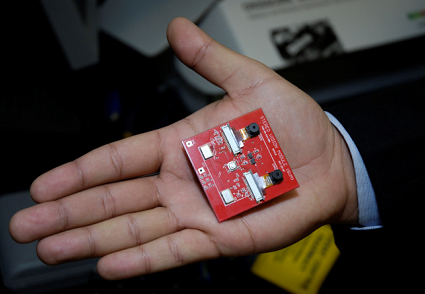
\includegraphics[width=\textwidth,height=4.5cm]{images/stoc_on_chip.png}
	 	\caption{Sistema de visão tridimensional
embarcado baseado em mapa de disparidade}
		\fonte{\cite{Khaleghi2008}}
	 	\label{fig:stoc_on_chip}
	\end{minipage}
	\hspace{0.1cm}
	\begin{minipage}[b]{0.55\linewidth}
	    \centering
	 	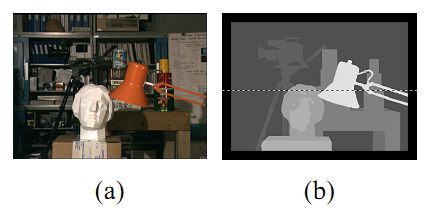
\includegraphics[width=\textwidth,height=4.5cm]{images/tsukuba.png}
	 	\caption{Estéreo: \textbf{(a)} imagem RGB \\ \textbf{(b)} disparidade referencial}
		\fonte{University of Tsukuba}
	 	\label{fig:tsukuba}
	\end{minipage}
\end{figure}

%Porém, essa não linearidade não é um artefato
%que resulta propriamente daquela implementação, 
%ela advém do fato de o mapa ser
%gerado a partir de imagens que são formadas pela projeção perspectiva que 
%inerentemente produz esse efeito (\textit{foreshortening}).

Em sistemas onde as câmeras são estacionárias (fixas em um local), como na
aplicação tradicional do Kinect, técnicas de extração e supressão do fundo podem
ser utilizadas para aumentar a robustez do método \cite{Ivanov2000}. No caso das
aplicações em robótica móvel, as câmeras estão em constante movimento
potencializando estes efeitos negativos, fazendo-se necessário outros métodos
para minimizar estes efeitos. Outra característica a ser apontada em relação ao
Kinect é sua inviabilidade de uso no ambiente externo, ou seja, com iluminação
natural - isto se deve ao fato da tecnologia empregada se basear em luz
estruturada e requer iluminação artificial (infra-vermelho) a qual sofre
interferência na presença de luz solar. Em ambiente externo são utilizadas
câmeras convencionais, onde o conjunto estéreo pode ser constituído tanto por
câmeras independentes permitindo maior versatilidade de poses como no uso de
câmeras do tipo STOC (\textit{STereo On a Chip}) que são mais estáveis em
relação à manutenção da calibragem.

%Em ambiente externo são utilizadas câmeras convencionais
%porém geralmente o uso de câmeras estéreo tipo STOC (\textit{STereo On a Chip})
%são um tipo de aplicação por serem mais estáveis em relação à manutenção da
%calibragem devido a vibrações.

%Fig. 2.7: Sistema de visão tridimensional
%embarcado baseado em mapa de disparidade
%Fonte: 
%Fig. 2.8: a) Imagem RGB; b) Mapa de disparidade Fonte: University of Tsukuba 

O mapa de disparidade provê uma percepção espacial que representa os elementos
da cena em um espaço tridimensional, fornecendo assim, uma fonte muito rica de
informações sobre a cena. A partir destas informações pode ser possível então
definir a trajetória do veículo de modo a desviar dos obstáculos que se
encontram a sua frente ao mesmo tempo em que este se locomove em direção ao seu
destino. Este processo é denominado de navegação robótica e será detalhado a
seguir.


%%2012-10-14 Lido OK
